\chapter{Enforcing Constraints}

This chapter explains how the constraints are expressed and validated with the tool. The constraints are divided into three distinct categories. The first category contains the constraints that are possible to express in ArchUnit as-is. The second category describes constraints that are enforceable with the help of additional information in source code. The third and final category details constraints that require an extension of ArchUnit to be possible to enforce.

\section{Support in ArchUnit as-is}\label{sec:as-is}

ArchUnit contains an extensive vocabulary for expressing typical architectural constraints. These constraints are generally composed of three parts. The first part indicates the type of Java construct that should be inspected. These constructs include classes, methods, fields and constructors. The second part contains a predicate that selects a subset of these constructs. The third part defines the condition that must hold true for all the selected constructs.

An example of a rule defined solely using this standard vocabulary can be seen in Listing~\ref{lst:standard_vocabulary}, where each of the three aforementioned parts of the constraint has been separated into their own line. The rule is a simple example of complete mediation, where some internal classes must only be accessed through a mediator.

\begin{minipage}{\linewidth}
\begin{lstlisting}[caption={Example of a rule that is expressed with the standard vocabulary.}, captionpos=b, label=lst:standard_vocabulary, numbers=left]
ArchRule rule = classes()
    .that().resideInAPackage("..internal..")
    .should().onlyBeAccessed().byAnyPackage("..mediator..");
\end{lstlisting}
\end{minipage}

In situations where this vocabulary is insufficient for expressing a constraint, there is a possibility to define custom predicates and conditions over any given construct. These can be supplied as arguments to the \texttt{that()} and \texttt{should()} methods. Custom predicates and conditions are used extensively in our implementation, as will be made apparent in the following sections.

\subsection{Log all security events}
% Description
This constraint is expressed with the assumption that there are services, in the form of classes, that are responsible for performing security related events. Any publicly accessible methods in these services perform a security event and must therefore contain a call to the logging facility.

% Rule definition
The definition of the architectural rule can be seen in Listing~\ref{lst:constraint_1_impl}. The predicate that selects the security services, and the class that is responsible for logging, are passed as arguments to the architectural rule. This leaves no need for injecting information into the source code of the target system. Furthermore, by using a predicate to select the security services, the developer is left with some flexibility in how they decide to apply the constraint. As opposed to a plain list of classes, a predicate can match all classes belonging to a specific package or following a set naming scheme, minimizing the need for revisiting the constraint as the system evolves.

\begin{minipage}{\linewidth}
\begin{lstlisting}[caption={Rule definition for constraint 1.}, captionpos=b, label=lst:constraint_1_impl, numbers=left]
ArchRule logSecurityEvents(
        DescribedPredicate<? super JavaClass> securityServicesDescriptor,
        Class<?> logger) {
    return methods()
        .that().haveModifier(JavaModifier.PUBLIC)
        .and().areDeclaredInClassesThat(securityServicesDescriptor)
        .should(callMethod(declaredIn(logger)));
}
\end{lstlisting}
\end{minipage}

% Applied to toy app
In the example system, illustrated in Figure~\ref{fig:toy_application}, the logging facility is the class named \texttt{Logger} while the only security service is the \texttt{UserService} class. An application of the constraint on this system can be as simple as the one shown in Listing~\ref{lst:constraint_1_toy}.

\begin{minipage}{\linewidth}
\begin{lstlisting}[caption={Application of constraint 1 to the example system.}, captionpos=b, label=lst:constraint_1_toy, numbers=left]
@ArchTest
ArchRule logSecurityEvents = SecArchUnit
    .logSecurityEvents(type(UserService.class), Logger.class);
\end{lstlisting}
\end{minipage}

\begin{figure}
    \centering
    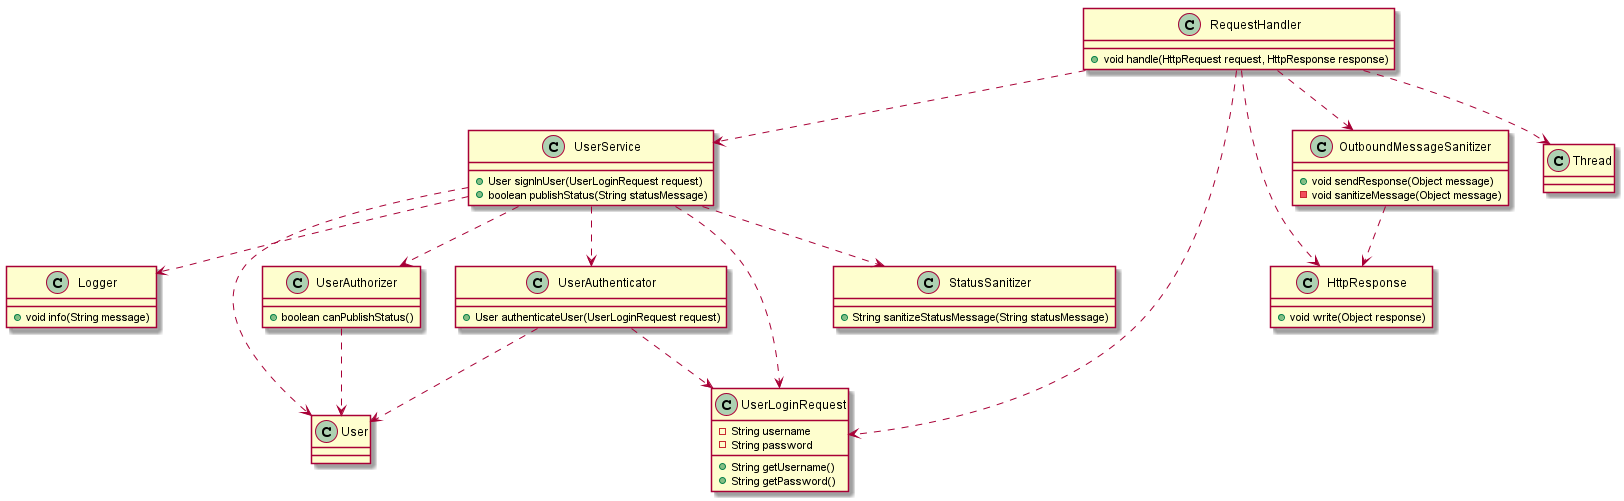
\includegraphics[width=\textwidth]{figure/ToyApp.png}
    \caption{An example of a system, for the purpose of illustrating how the constraints are applied.}
    \label{fig:toy_application}
\end{figure}

\subsection{Enforce AuthN/AuthZ at single point}
% Description
The second constraint is defined in terms of two concepts: an authentication point and an authentication enforcer. Authentication is performed through a method call to the authentication enforcer, which is a class whose sole responsibility is to authenticate an actor. This call should occur at the authentication point, and at no other points in the system, for the sake of ensuring a uniform authentication mechanism throughout the system. Authorization is enforced in the same manner, with the concepts of an authorization point and an authorization enforcer.

% Rule definition
The definition of the second constraint is detailed in Listing~\ref{lst:constraint_2_impl}. The constraint is defined as two separate rules, for the sake of clarity, but their implementations are identical.

\begin{minipage}{\linewidth}
\begin{lstlisting}[caption={Rule definition for constraint 2.}, captionpos=b, label=lst:constraint_2_impl, numbers=left]
ArchRule enforceAuthenticationAtCentralPoint(
        Class<?> authenticationPoint,
        Class<?> authenticator) {
    return CompositeArchRule.of(
        theClass(authenticationPoint)
            .should(callMethod(declaredIn(authenticator)))
    ).and(
        methods()
            .that().areDeclaredIn(authenticator)
            .should(onlyBeAccessedBy(authenticationPoint))
    );
}

ArchRule enforceAuthorizationAtCentralPoint(
        Class<?> authorizationPoint,
        Class<?> authorizer) {
    return enforceAuthenticationAtCentralPoint(
        authorizationPoint,
        authorizer
    );
}
\end{lstlisting}
\end{minipage}

% Applied to toy app
In the example system, the authentication and authorization points are both situated in the \texttt{UserService} class while authentication and authorization are enforced by the classes \texttt{UserAuthenticator} and \texttt{UserAuthorizer} respectively. The application of the rule can be seen in Listing~\ref{lst:constraint_2_toy}.

\begin{minipage}{\linewidth}
\begin{lstlisting}[caption={Application of constraint 2 to the example system.}, captionpos=b, label=lst:constraint_2_toy, numbers=left]
@ArchTest
ArchRule enforceAuthentication = SecArchUnit
    .enforceAuthenticationAtCentralPoint(UserService.class, UserAuthenticator.class);

@ArchTest
ArchRule enforceAuthorization = SecArchUnit
    .enforceAuthorizationAtCentralPoint(UserService.class, UserAuthorizer.class);
\end{lstlisting}
\end{minipage}

\subsection{Messages are sent from a central point}
% Description
The third constraint dictates that all outbound messages are sent from a central sending point. The intent is to have a single point that handles output sanitization or performs other safety checks on messages before they are sent. The act of sending a message is defined as a method call to a sender with at least one argument, which is assumed to contain the message contents. The reasoning is that any class should be allowed to create and pass around a sender instance without violating the constraint.

% Rule definition
The rule definition can be seen in Listing~\ref{lst:constraint_3_impl}. Since there can be multiple sender classes in a system, e.g. one for HTTP requests and one for SMTP messages, the rule accepts a predicate that can select all these sender classes.

\begin{minipage}{\linewidth}
\begin{lstlisting}[caption={Rule definition for constraint 3.}, captionpos=b, label=lst:constraint_3_impl, numbers=left]
ArchRule sendOutboundMessagesFromCentralPoint(
        Class<?> sendingPoint,
        DescribedPredicate<? super JavaClass> senderDescriptor) {
    return methods()
        .that().areDeclaredInClassesThat(senderDescriptor)
        .and(haveAtLeastOneParameter)
        .should(onlyBeAccessedBy(sendingPoint));
}
\end{lstlisting}
\end{minipage}

% Applied to toy app
Listing~\ref{lst:constraint_3_toy} showcases how the constraint can be applied to the example system. In this system, there is a single sender class \texttt{HttpResponse}, responsible for returning a response to a client. The central sending point is the \texttt{OutboundMessageSanitizer} class. 

\begin{minipage}{\linewidth}
\begin{lstlisting}[caption={Application of constraint 3 to the example system.}, captionpos=b, label=lst:constraint_3_toy, numbers=left]
@ArchTest
ArchRule centralSendingPoint = SecArchUnit
    .sendOutboundMessagesFromCentralPoint(
        OutboundMessageSanitizer.class,
        type(HttpResponse.class)
    );
\end{lstlisting}
\end{minipage}




\section{Injecting Information into Source Code}

Some of the architectural constraints require that the developer injects additional information into the source code. In some cases, this information is simply an indicator that says something about an entire class. Naming the class with a specific suffix is one approach to accomplish this. Another approach is to implement an empty interface, which is the technique used with Java's \texttt{Serializable}\footnote{https://docs.oracle.com/javase/7/docs/api/java/io/Serializable.html} interface. 

In other cases, however, the information may be required for methods of arbitrary signatures and even specific fields. For the purposes of flexibility and minimizing the obtrusiveness of our approach, any extra information is expressed in the form of annotations. These can be applied to classes, fields, methods and parameters without changing the underlying architecture of the system.

The need for additional information within the source code becomes apparent in the case where a class contains public methods with varying degrees of security requirements. A typical example is found in constraint 4, where a class is responsible for handling user input. Some methods might receive predefined values, such as in the case of checkboxes, whereas others treat strings entered by the user.  The former type of input is guaranteed to be safe, whereas the latter entirely under the control of the attacker, thus introducing the need for sanitation. Using the broader predicate of entire classes (described in section \ref{sec:as-is}) would not allow the constraint to be limited to specific methods within a class (those receiving potentially malicious input), and later trace a call to a method providing sanitation. Thus, annotations provide the granularity needed to limit the scope of a constraint to only the applicable code units.

\todo{Specific example that requires additional information}

\todo{Show rule definition for each constraint}
\todo{Show how each constraint is used in our toy app}

\subsection{Validate user input}
User input comes in many forms, and as such, it is impossible to define a single algorithm to validate properly every single type. The problem grows further as queries (such as SQL) or other types of processed data (such as XML), each with its own set of grammar, are often formed using strings. As a consequence, the implemented constraint is more abstract as it checks whether a class that receives user input is said to either perform validation on its own or delegate the task another method. In total, four distinct cases conforming to the constraint where considered: 

\begin{itemize}
    \item \textit{Method A} is annotated with both \textbf{UserInput} and \textbf{InputValidator}.
    
    \item \textit{Method A} is annotated with \textbf{UserInput} and calls a \textit{method B} that is annotated with \textbf{InputValidator}.
    
    \item \textit{Method A} is annotated with \textbf{UserInput} and is only called by methods that are annotated with \textbf{InputValidator}.
    
    \item \textit{Method A} is annotated with \textbf{UserInput} but is never called.
\end{itemize}

The rule definition can be seen in Listing \ref{lst:constraint_4_impl}. As shown, the \textbf{UserInput} annotation is used on line 3 to limit the set of applicable code units, whereas the custom condition \texttt{performDirectOrIndirect} implements the logic to detect violations for each of the four cases outline above.
    
\begin{minipage}{\linewidth}
\begin{lstlisting}[caption={Rule definition for constraint 4.}, captionpos=b, label=lst:constraint_4_impl, numbers=left]
public static ArchRule validateUserInput() {
    return codeUnits()
        .that().areAnnotatedWith(UserInput.class)
        .should(performDirectOrIndirectValidation);
}
\end{lstlisting}
\end{minipage}

In the example system, a user publishes a status update in the form of a string that the UserService class receives. The status is then passed to the StatusSanitizer class, where it is validated. The affected methods of each class are marked with the appropriate annotation, as shown in figure \ref{fig:validate_input_toy_system}.  

\begin{figure}
    \centering
    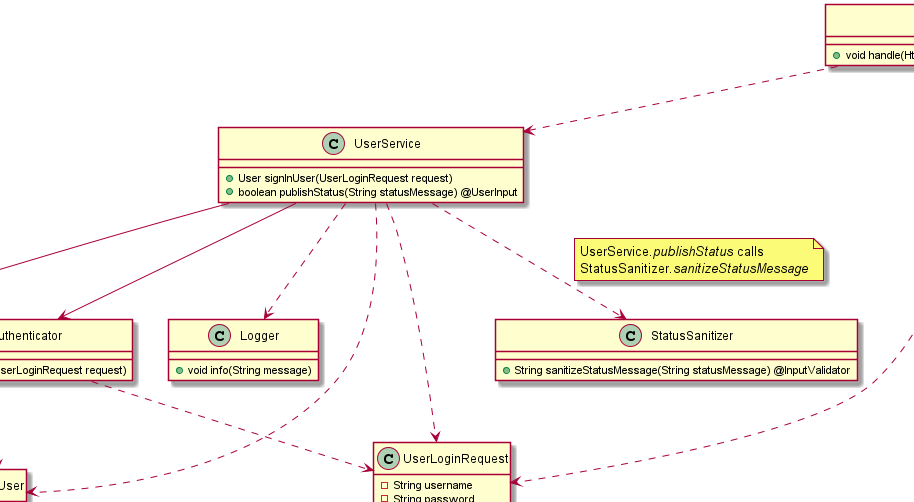
\includegraphics[width=\textwidth]{figure/toyexamples/validate_input_toy_system.png}
    \caption{Applying constraint 4 to the model of the example system using added annotations.}
    \label{fig:validate_input_toy_system}
\end{figure}

\subsection{Restrict thread spawning}
While resources is a broad term, this constraint focuses on preventing the exhaustion of CPU and memory resources through the creation of new threads and processes. As such, every block of code that contains a call to the \texttt{start()} method of a \texttt{Thread}\footnote{\url{https://docs.oracle.com/javase/7/docs/api/java/lang/Thread.html}} or any of its subclasses, must be marked as containing a resource restriction mechanism. The same rule is applied for calls to \texttt{ProcessBuilder.start()}\footnote{\url{https://docs.oracle.com/javase/7/docs/api/java/lang/Process.html}} and \texttt{Runtime.exec()}\footnotemark[3], which lead to the creation of new processes.
% TODO manual footnote, adjust as necessary

The marking is done with the help of an annotation, either on the relevant method or the entire class. The decision of how the restriction mechanism is implemented is left to the developer of the system.

\begin{minipage}{\linewidth}
\begin{lstlisting}[caption={Rule definition for constraint 5.}, captionpos=b, label=lst:constraint_5_impl, numbers=left]
public static ArchRule limitResourceAllocation() {
    return noClasses()
        .that().areNotAnnotatedWith(ResourceRestriction.class)
        .should().callMethodWhere(
            aThreadIsStartedWithoutRestriction
        ).orShould().callMethodWhere(
            aProcessIsStartedWithoutRestriction
        );
}
\end{lstlisting}
\end{minipage}




\section{Extending ArchUnit Analysis}

In the current ArchUnit API, a rule that aims to constrain method calls can only be defined in terms of the type signatures of the method and its parameters. This is a non-issue when the arguments being passed to a method are of the same type as the parameters. However, in cases where a method parameter accepts a "more general" type, such as an \texttt{Object}, there is no way for ArchUnit to constrain the types of the objects that are actually being passed as arguments.

Consider constraint 7, which aims to ensure that no secrets are passed to the logger. Say there is a \texttt{Secret} annotation that marks all the classes whose instances must not be passed to the logger. We can attempt to enforce the constraint with the current ArchUnit API and a few custom predicates, as seen in Listing~\ref{lst:constraint_6_attempt}. However, a typical logger class will accept either a plain string, or a format string along with an array of objects to be formatted. In such cases, this architectural rule will be unable to catch secrets that are passed to the logger.

\begin{minipage}{\linewidth}
\begin{lstlisting}[caption={A first attempt to implement constraint 7.}, captionpos=b, label=lst:constraint_6_attempt, numbers=left]
public static ArchRule doNotLogSecrets(Class<?> logger) {
    return noClasses()
        .should().callMethodWhere(
            parameterTypeAnnotatedWith(Secret.class)
                .and(targetOwner(type(logger)))
        );
}
\end{lstlisting}
\end{minipage}

For the final 2 constraints, there is a need for an extension that allows constraints to be defined against arguments, rather than parameters. There should also be hints about where these arguments may have been derived from, e.g. which types that make up the components of a concatenated string. In the following sections, we will describe the extensions that have been made to ArchUnit and how these are utilized in the definitions of our constraints.

\subsection{Extensions}
\todo{Parts of this section probably belong in the background}

ArchUnit builds its representation of the architecture using ASM\footnote{\url{https://asm.ow2.io/}}, a Java bytecode analysis framework. ASM reads bytecode and generates callbacks to methods in its various visitor classes\footnote{\url{https://asm.ow2.io/javadoc/org/objectweb/asm/package-summary.html}}. The visitor of most interest to us is \texttt{MethodVisitor}, which is responsible for processing the contents of a method, constructor or static initializer. These are collectively named \textit{code units} in ArchUnit's domain, i.e. anything that contains code. 

ArchUnit extends the \texttt{MethodVisitor} class in \texttt{MethodProcessor} and translates the instructions into information about field accesses, method invocations, et. cetera, building its representation of the architecture. A short excerpt of the various callbacks available to this visitor can be seen in Figure~\ref{fig:method_processor_1}. The class \texttt{MethodProcessor} extends

\begin{figure}
    \centering
    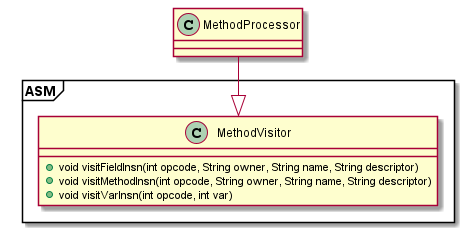
\includegraphics[width=0.6\textwidth]{figure/extension/MethodProcessor1.png}
    \caption{The immediate context of the \texttt{MethodProcessor} class in ArchUnit, responsible for processing bytecode instructions.}
    \label{fig:method_processor_1}
\end{figure}


Java is a stack-oriented programming language, meaning that arguments to method calls and field assignments are passed via the stack \cite{hutchison_information_2005}. As such, inspecting the stack at the time of a method call or field assignment will allow us to learn the types of the arguments that are being passed.

\begin{figure}
    \centering
    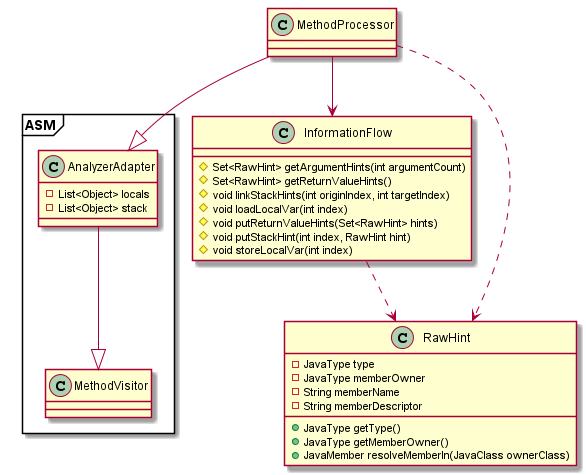
\includegraphics[width=0.8\textwidth]{figure/extension/MethodProcessor2.png}
    \caption{Changes made to the \texttt{MethodProcessor} class and its surroundings.}
    \label{fig:method_processor_2}
\end{figure}

\todo{describe our information flow analysis, reference existing approaches}

\todo{Diagram of changes to ArchUnit domain}

Our extension provides this additional information in ArchUnit's representation of accesses to fields and methods, which the rule definitions can then make use of.


\todo{Detail the extensions we made}

\todo{Show rule definition for each constraint}
\todo{Show how each constraint is used in our toy app}

\subsection{Sensitive information must stay within trust boundary}
...

\subsection{Secrets must not be exposed in log messages}
...
